No que diz respeito a algoritmos de aproximação, \citeauthor{li2002closest} propôs, e demonstrou, uma aproximação em tempo polinomial com razão de aproximação $1 + \epsilon$ para o problema da \textit{closest string} \cite{li2002closest}, como descrito na Tarefa 1.
A implementação do algoritmo não é trivial e acredito que esteja um pouco além do que é requerido por este trabalho. Além disso, não existe uma implementação desse algoritmo acessível, então decidi por não me estender muito nesse resultado.

Vamor propor e implementar, nesta tarefa, um algoritmo no estilo \textit{branch and bound}, que nos permita explorar todas as soluções, porém ignorar aquelas em que temos certeza que não são boas o suficiente. Imagine que o Algoritmo \ref{alg:exact} funcione a partir de ramificações. Ou seja, o primeiro nó da árvore é vazio e possui como filhos todas as possibilidades para a primeira letra; escolhido um filho, seus filhos possuem todas as possibilidades para a segunda letra; e assim por diante, como na \autoref{fig:tree}. Esse é o \textit{branch}.

\begin{figure}[H]
    \centering
    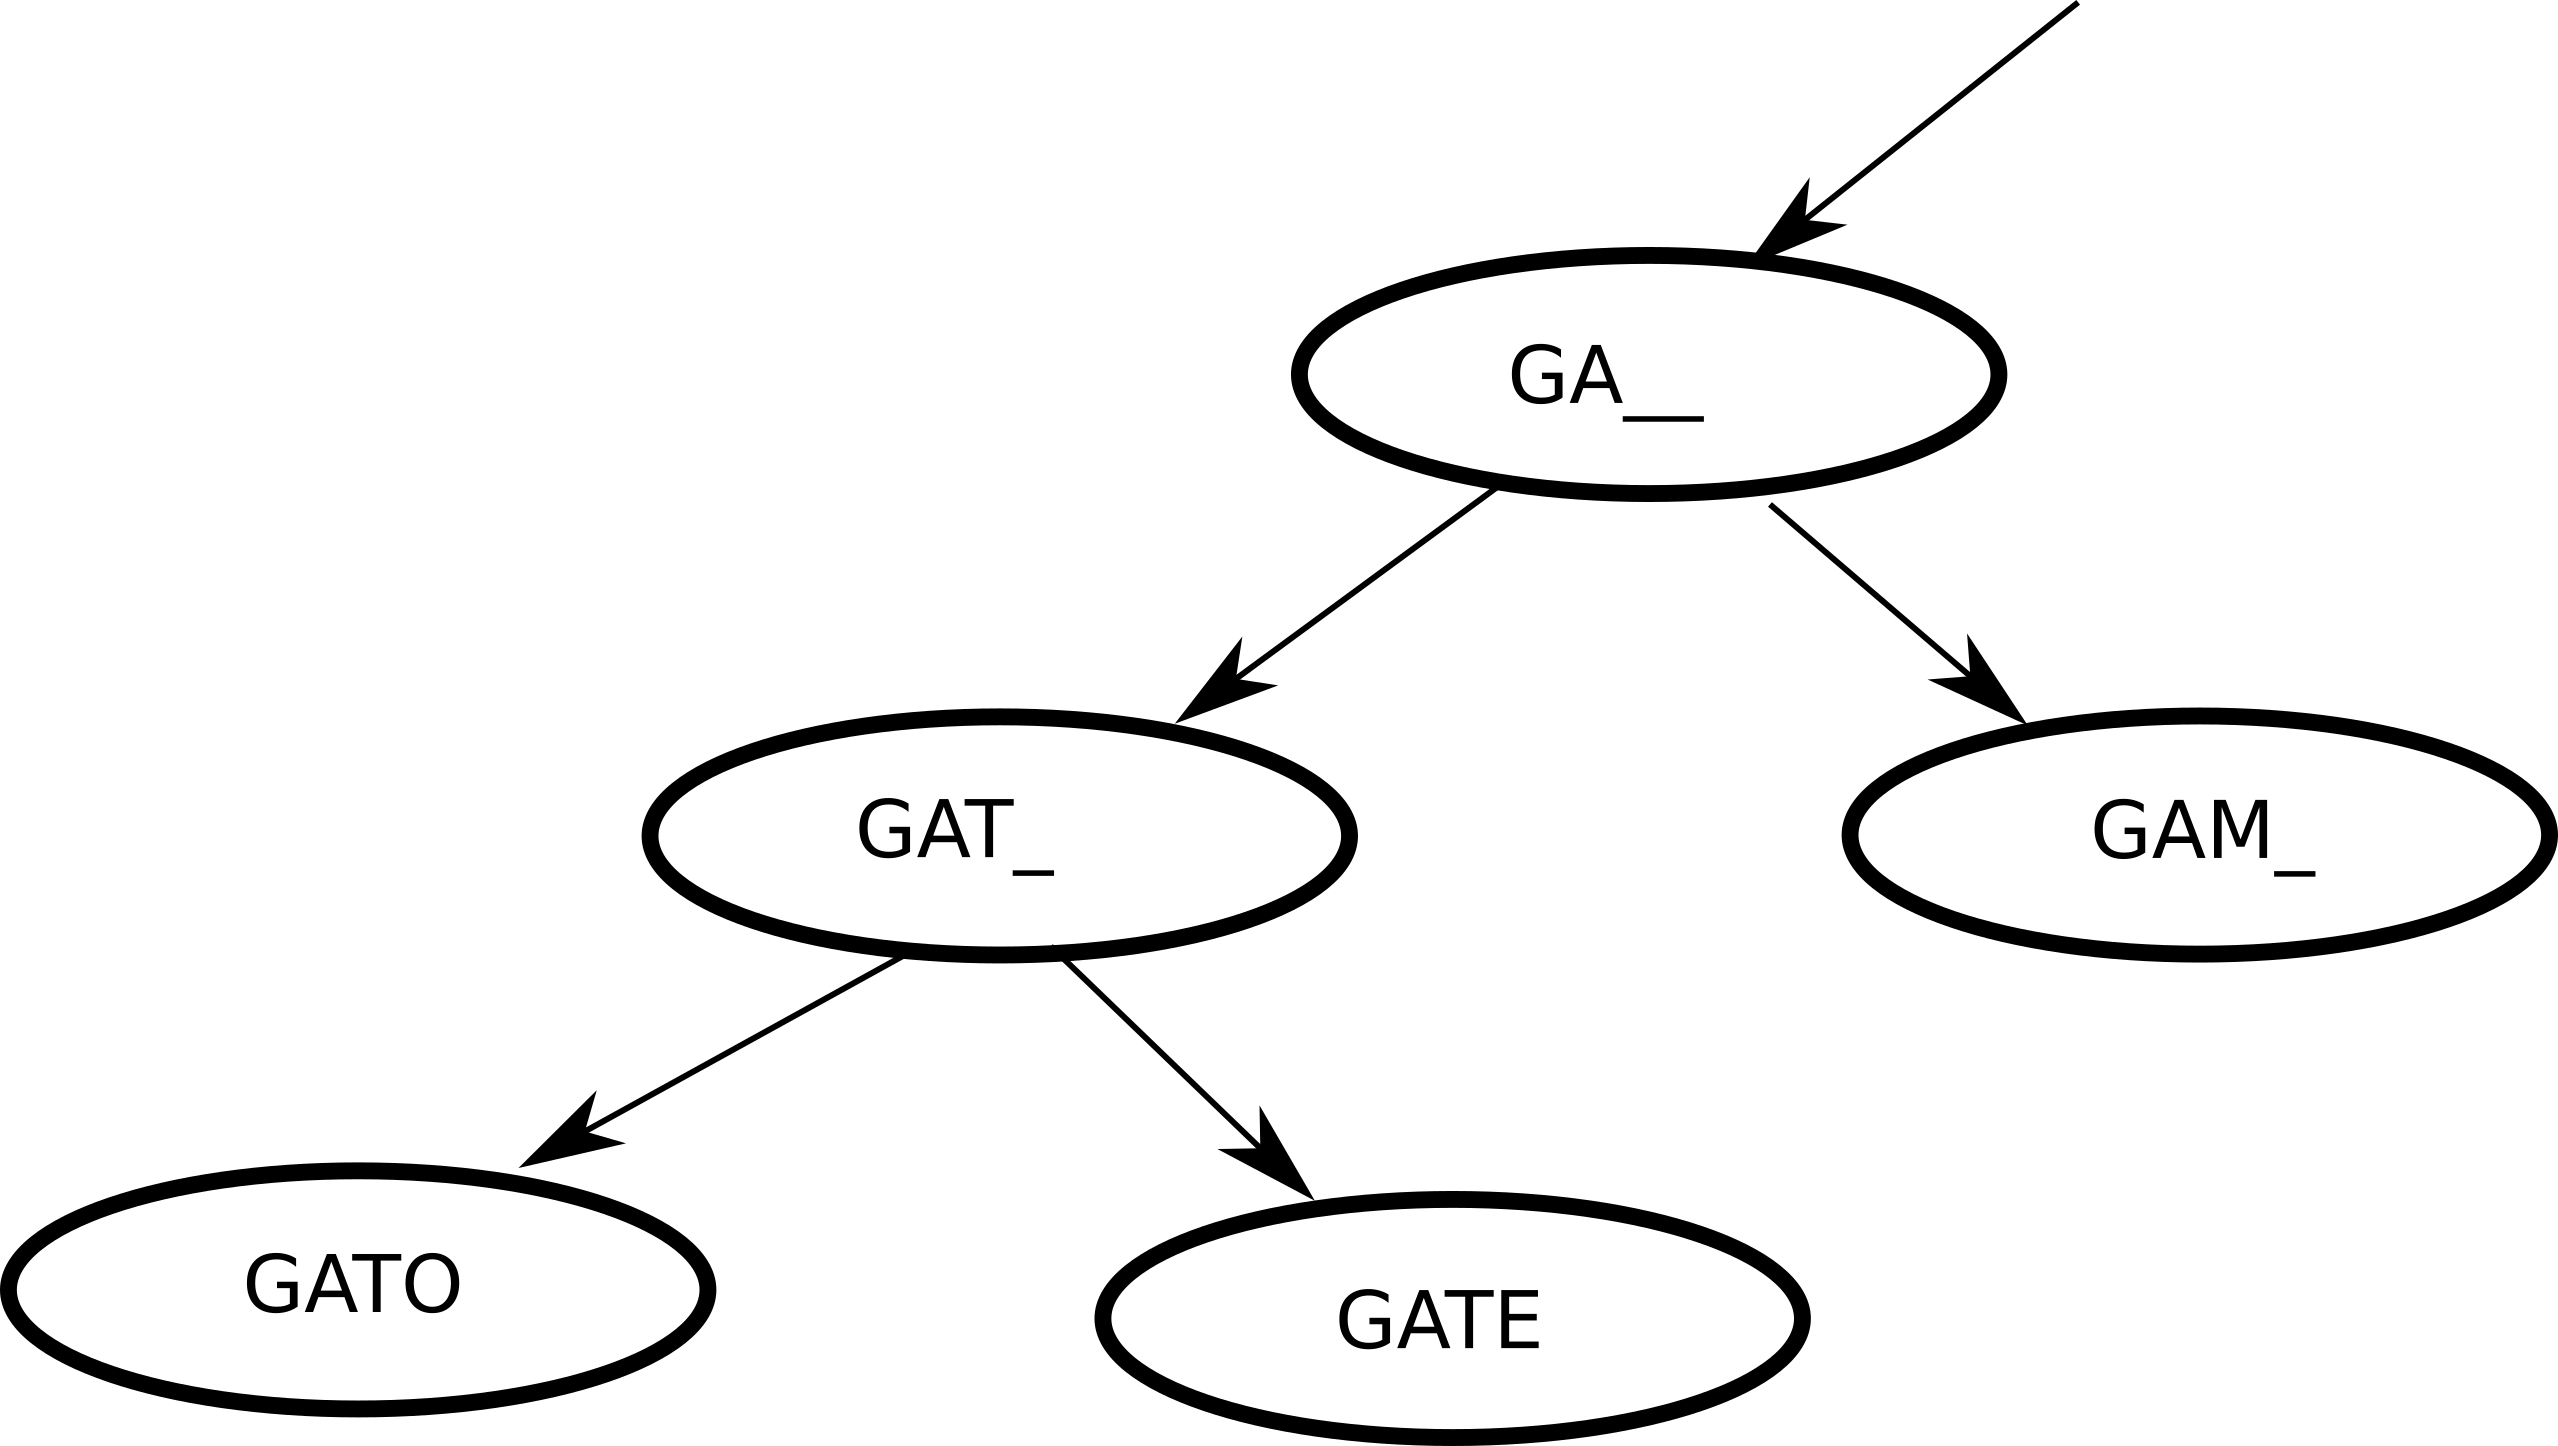
\includegraphics[width=0.6\linewidth]{tree.png}
    \caption{Exemplo de árvore.}
    \label{fig:tree}
\end{figure}

Para saber se é válido explorar uma subárvore, isto é, quando realizar o \textit{bound}, vamos utilizar um \textit{lower bound} para o menor custo $d$ em uma subárvore. Note que, em um nó com as $i$ primeiras letras definidas, temos o custo dessas $i$ primeiras letras já calculado; precisamos nos preocupar apenas com as $m-i$ letras restantes, isto é, $s[i+1:m]$. Note que, se quisermos minimizar a soma das distâncias de Hamming de $s[i+1:m]$ às strings $s_1[i+1:m], \cdots, s_n[i+1:m]$, basta que tomemos, em cada posição, aquela letra mais comum para aquela posição. Seja essa a string $s^\ast$. Ora, se $d_{OPT}$ é custo mínimo ótimo para as strings $s_1[i+1:m], \cdots, s_n[i+1:m]$, com centro $s^{\ast\ast}$, então vale que $\text{d}(s^{\ast\ast}, s_i[i+1:m]) \le d_{OPT}$ para todo $j$, de forma que
\[\sum_j \text{d}(s^{\ast\ast}, s_j[i+1:m]) \le n d_{OPT},\]
e, finalmente,
\[\frac{\sum_j \text{d}(s^{\ast}, s_j[i+1:m])}{n} \le \frac{\sum_j \text{d}(s^{\ast\ast}, s_j[i+1:m])}{n} \le d_{OPT},\]
sendo a primeira desigualdade justificada pelo fato de que $s^\ast$ minimiza a soma das distâncias de Hamming.
Ou seja, a soma das distâncias de Hamming a $s^\ast$ (a string de $i+1$ a $m$ que toma as letras mais comuns) sobre $n$ é um lower bound para o custo ótimo de uma subárvore, ignorando as $i$ primeiras posições. Isso, somado ao custo das $i$ primeiras posições, nos dá um \textit{lower bound} para o custo ótimo de uma subárvore. Sendo assim, não precisamos explorá-la caso já tenhamos uma solução melhor.
O Algoritmo \ref{alg:tree} descreve um pseudocódigo para essa solução.

\begin{algorithm}[H]
    \caption{Algoritmo \textit{branch and bound} para o problema da \textit{closest string}.}
    \label{alg:tree}
    \begin{algorithmic}
        \Require Strings $s_1, \cdots, s_n$ de tamanho $m$
        \State Cria os conjuntos $S_i = \left\{s_1[i], \cdots, s_n[i]\right\}$, para cada $i$
        \State Inicializa uma solução qualquer $s_0$
        \State Calcula o valor $d_0$ da solução $s_0$
        \State $s \gets$ empty string
        \State $\textsc{branch}(s)$        
        \State \Return $s_0, d_0$
        \State
        \Procedure{branch}{$s$}
            \State $i = \text{length}(s)$
            \If{$i=m$}
                \State $d \gets$ custo de $s$
                \If{$d < d_0$}
                    \State $s_0 \gets s$
                    \State $d_0 \gets d$
                \EndIf
                \State \Return
            \EndIf
            \State $l \gets$ \textit{lower bound} para o custo mínimo de $s$ \Comment{Aqui usamos o que foi descrito na solução.}
            \If{$l > d_0$}
                \State \Return
            \EndIf
            \For{char $\in S_i$}
                \State $\textsc{branch}(s + \text{char})$ \Comment{Estamos adicionando char à string $s$.}
            \EndFor
        \EndProcedure
    \end{algorithmic}
\end{algorithm}

A implementação do Algoritmo \ref{alg:tree} for realizada em Python, podendo ser conferida \href{https://github.com/lucasresck/data-structures-algorithms/blob/main/intractable_problems/scripts/closest_string_tree.py}{neste link}. Por exemplo, se pedirmos ao programa qual a \textit{closest string} para 
\[\overset{\underbrace{\text{\fbox{G}\fbox{A}\fbox{T}\fbox{O}}\cdots\text{\fbox{G}\fbox{A}\fbox{T}\fbox{O}}}}{\text{8 vezes}}\]
\[\overset{\underbrace{\text{\fbox{G}\fbox{A}\fbox{M}\fbox{E}}\cdots\text{\fbox{G}\fbox{A}\fbox{M}\fbox{E}}}}{\text{8 vezes}}\]
\[\overset{\underbrace{\text{\fbox{G}\fbox{A}\fbox{M}\fbox{O}}\cdots\text{\fbox{G}\fbox{A}\fbox{M}\fbox{O}}}}{\text{8 vezes}}\]
obtemos 
\[\overset{\underbrace{\text{\fbox{G}\fbox{A}\fbox{M}\fbox{O}}\cdots\text{\fbox{G}\fbox{A}\fbox{M}\fbox{O}}}}{\text{8 vezes}}\] em 28779 iterações. Um ponto importante é que, sem o \textit{bound}, esse número se torna 174761, significantemente maior.

A corretude do algoritmo é direta, pois é herdada do algoritmo da Tarefa 2 (que é exato) juntamente com a corretude do \textit{bound}, como discutido anteriormente. Porém, esse processo de \textit{bound} não garante que um número significativo de casos será eliminado: ainda, no pior caso, poderíamos passar por todos os nós.
Note que nosso Algoritmo \ref{alg:tree} é essencialmente o Algoritmo \ref{alg:exact}, porém no formato de árvore (com recursões), além do fato de que são calculados os lower bounds. O cálculo do lower bound tem complexidade $O(mn + m)$\footnote{Para perceber isso, veja que a primeira parcela se refere ao custo atual até a posição $i$, enquanto a segunda parcela se refere ao lower bound a partir da posição $i+1$. Esse custo é linear, pois é possível ter os ``custos de cada posição'' previamente calculados. Para mais detalhes, por favor, conferir a implementação.}.
Como a quantidade de nós é $O(|\Sigma|^{m})$\footnote{Não queria me estender aqui, porém a quantidade de nós pode ser dada por, no pior caso, $0 + |\Sigma| + \cdots + |\Sigma|^m = \frac{|\Sigma|^{m+1}-|\Sigma|}{|\Sigma| - 1} \le \frac{|\Sigma|^{m+1}}{|\Sigma| - 1} = O(|\Sigma|^m)$, pois $\Sigma$ é fixo.}, isso faz com que a complexidade do algoritmo continue a mesma da Tarefa 2: $O(mn|\Sigma|^{m})$.
